\chapter{Resultados}
\label{chapter:Resultados}

Una vez detectadas las anomalías se generan un fichero con solo las anomalías detectadas para cada ventana de tiempo. Sobre un a cantidad total de 46713 conexiones formadas tanto por conexiones de origen y destino, las anomalías detectadas por cada ventana son las siguientes:

\begin{table}[H]
    \centering
    \begin{tabular}{|c|c|c|c|}
    \hline
    \; & 30 min & 10 min & 5 min \\ [0.5ex]
    \hline
        \textbf{Columnas} & 1102 & 3202 & 6310 \\
        \hline
        \textbf{Anomalías} & 368 & 387 & 396 \\ [1ex]
    \hline
    \end{tabular}
    \caption{Anomalías por ventana de tiempo}
    \label{tab:results}
\end{table}

Haciendo una comparación entre las distintas anomalías y las distintas ventanas se encuentra que:
\begin{itemize}
    \item La cantidad de anomalías coincidentes entre las ventanas de 30 y 5 minutos es de 362
    \item La cantidad de anomalías coincidentes entre las ventanas de 10 y 5 minutos es de 383
    \item La cantidad coincidente entre todas las ventanas es de 360
    \item La evaluación principal se desarrollará sobre la ventana de 5 minutos, al contener la mayoría de anomalías
\end{itemize}

La evaluación y la comparación de resultados se dificulta al no tener un conjunto de datos etiquetados con el que comparar, por lo que se realiza un análisis sobre las variables comparando los valores anómalos con un muestreo de un 20\% de los datos originales no anómalos, dividido en conexiones origen y destino. La comparación se realiza visualmente evaluando la evolución de las conexiones según la variable a lo largo del periodo, estas visualizaciones no se van a mostrar en este capítulo de la memoria debido a longitud y cantidad de visualizaciones, pero se encuentra disponible en el \href{https://github.com/Gonmeso/TFM_Anomaly_Detection/blob/master/models/Anomaly_Detection_Evaluation.ipynb}{repositorio}  asociado al trabajo o en el anexo \ref{appendix}. Para cada variable se analizan las agregaciones por separado. Un ejemplo de las visualizaciones utilizadas es la siguiente:

\begin{figure}[h]
    \centering
    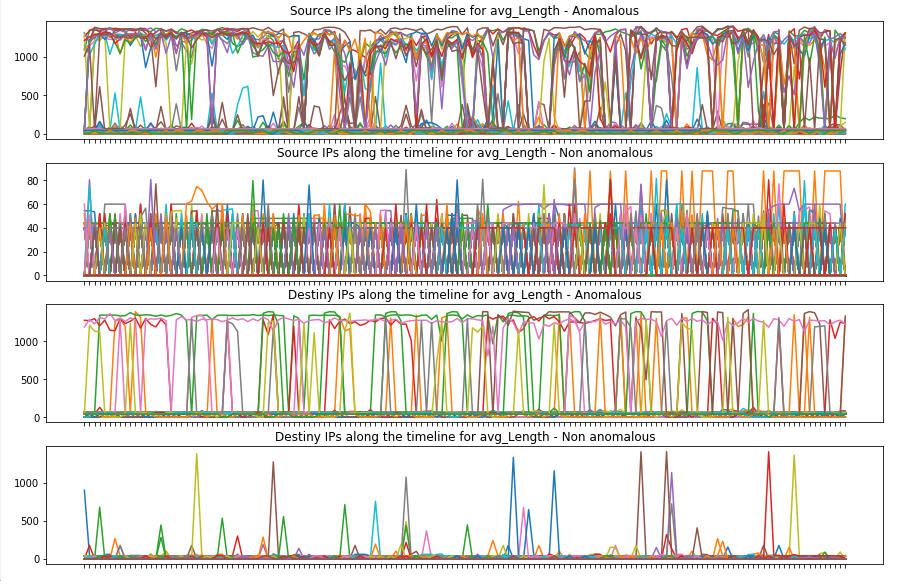
\includegraphics[width=17cm]{figs/evalutaion_example.PNG}
    \caption{Visualización de evaluación para la media de la variable \textit{Length}}
    \label{fig:eval_example}
\end{figure}

Para la variable \textit{Length} se puede observar lo siguiente:
\begin{itemize}
    \item La media en las conexiones de origen  tiene más variación que las no anómalas.
    \item Las no anómalas por lo general tienen valores medios muy pequeños.
    \item Para las conexiones de destino también existen conexiones con valores grandes, pero la mayoría tienen valores pequeños.
    \item Por lo general la media es mayor en las conexiones anómalas, puede tratarse de inyección de \textit{malware} por ejemplo.
    \item La desviación estándar tiene valores más altos por lo general para los anómalos, al contrario de las no anómalas que tiene valores muy pequeños.
    \item El sumatorio de los valores es mucho más alto en anómalos y muy bajo en comparación con los no anómalos.
    \item Ciertas representaciones coinciden tanto para destino como origen, lo que puede significar conexiones asiduas entre ambas IPs.
\end{itemize}

Para la variable \textit{IP1\_IP2\_time\_diff\_per\_value} (la diferencia de tiempos entre conexiones únicas de origen y destino) se puede observar lo siguiente:
\begin{itemize}
    \item Se presenta un patrón temporal para la media.
    \item Las conexiones anómalas tienen medias mayores.
    \item El patrón temporal también se aprecia en la desviación estándar.
    \item Los tiempos en las no anómalas en su mayor parte son muy pequeños.
    \item El sumatorio es mayor en anómalos.
\end{itemize}

Para la variable \textit{IP1\_time\_diff\_per\_value} (la diferencia de tiempos entre conexiones únicas de origen) se observa un patrón temporal en las conexiones destino, pero no en las de origen para los valores medios. Para \textit{IP2\_time\_diff\_per\_value} se observa el mismo patrón pero cambiado a las conexiones origen. Por otro lado, la distancia entre IPs, parece mostrar que las conexiones anómalas, tanto para origen como destino, pueden provenir de redes más cercanas.

En resumen para las variables de la cantidad de puertos en el último minuto se puede encontrar lo siguiente:

\begin{itemize}
    \item Se tiene, de media, un mayor uso de puertos de destino en las conexiones anómalas, mucho más grande para las conexiones de destino que las de origen.
    \item Para las observaciones no anómalos por lo general la cantidad de puertos de origen es muy baja.
    \item Destaca mucho la cantidad de puertos de origen que se utilizan en las conexiones de destino.
    \item Para la cantidad de puertos de destino, es claramente mayor para conexiones origen en los valores anómalos, lo que significa que esas IPs pueden estar haciendo escaneos.
    \item La suma de puertos de destino para las conexiones de origen anómalas es muy grande en comparación al resto. 
\end{itemize}

En las variables binarias se puede observar que la conexión tenga un valor positivo en alguna de ellas puede favorecer a considerarlo como anómalo. Tal y como se comentó con anterioridad, estos pueden ser comandos que se utilicen para infectar los dispositivos, por lo que puede tener sentido.

En resumen las anomalías presentan los siguientes rasgos:

\begin{itemize}
    \item Mayores tiempos de diferencias entre conexiones (es decir, el tiempo que ha tardado en volver a conectarse), siguiendo cierto patrón.
    \item Mayor cantidad de puertos de origen y destino utilizados que las conexiones no anómalas.
    \item Mayor cantidad de información en los paquetes transmitida que los no anómalos.
    \item Cuentan con un pequeño porcentaje mayor de is\_busybox e is\_enable" que los no anómalos, pero muy pequeño.
    \item Las conexiones pueden tener cierta periodicidad en conexiones únicas de IP origen e IP destino, pero las origen siguen realizando conexiones a otros destinos.
    \item Una mayor cantidad de puertos destinos, puede indicar un escaneo.
    \item Mayor cantidad de información transmitida puede presentarse como inyección de \textit{malware}.
\end{itemize}